% 原章第71—75页附录标题前：例6.6，6.7，软件，式6.242—6.243。
\Needspace{4\baselineskip}
\noindent\textbf{例 6.6}

为评价所提模型用于 fMRI 有效连接分析的可行性，将整数规划（IP）用于从公共数据仓库 OpenfMRI（\url{https://openfmri.org/}）下载的 6 名个体的静息 fMRI 数据。稀疏时间序列 SEM 作为定义评分函数与因果图学习超结构的工具。fMRI 数据采用事件相关设计的气球模拟风险任务采集。fMRI 测量持续 200 秒，单帧图像维数为 $64*64*10$。利用简单线性迭代聚类（simple linear iterative clustering，SLIC）超体素算法，将脑分割为 34 个子区域，以各子区域总体积作为影像信号度量。

图 6.15 给出静息 fMRI 的有效连接结果，只显示皮质区域之间的连接，其他区域未显示。图中呈现时刻 $t-1$ 与 $t$ 之间变化的脑有效连接模式。时刻 $t-1$ 的“额上区 $\to$ 眶额区”“颞中区 $\to$ 额下区”“颞上区 $\to$ 颞中区”，在时刻 $t$ 仍然存在；时刻 $t-1$ 的“额上区 $\to$ 中央区 $\to$ 颞上区”，变为“额上区 $\to$ 颞上区”。时刻 $t-1$ 的“枕区 $\to$ 颞上区”，在时刻 $t$ 消失。从时刻 $t-1$ 到时刻 $t$，“额上区 $\to$ 中央区”与“上区 $\to$ 颞中区”这两个方向来自时刻 $t-1$ 的方向，而“额下区 $\to$ 颞上区”及“眶额区 $\to$ 中央区”则是新形成的方向。
% 原脑影像/全部连边与颜色保留；中文标签在原PDF文字层对应位置覆盖。
\begin{figure}[htbp]
\centering
\begin{tikzpicture}[x=1cm,y=1cm]
\node[anchor=south west,inner sep=0] at (0,0) {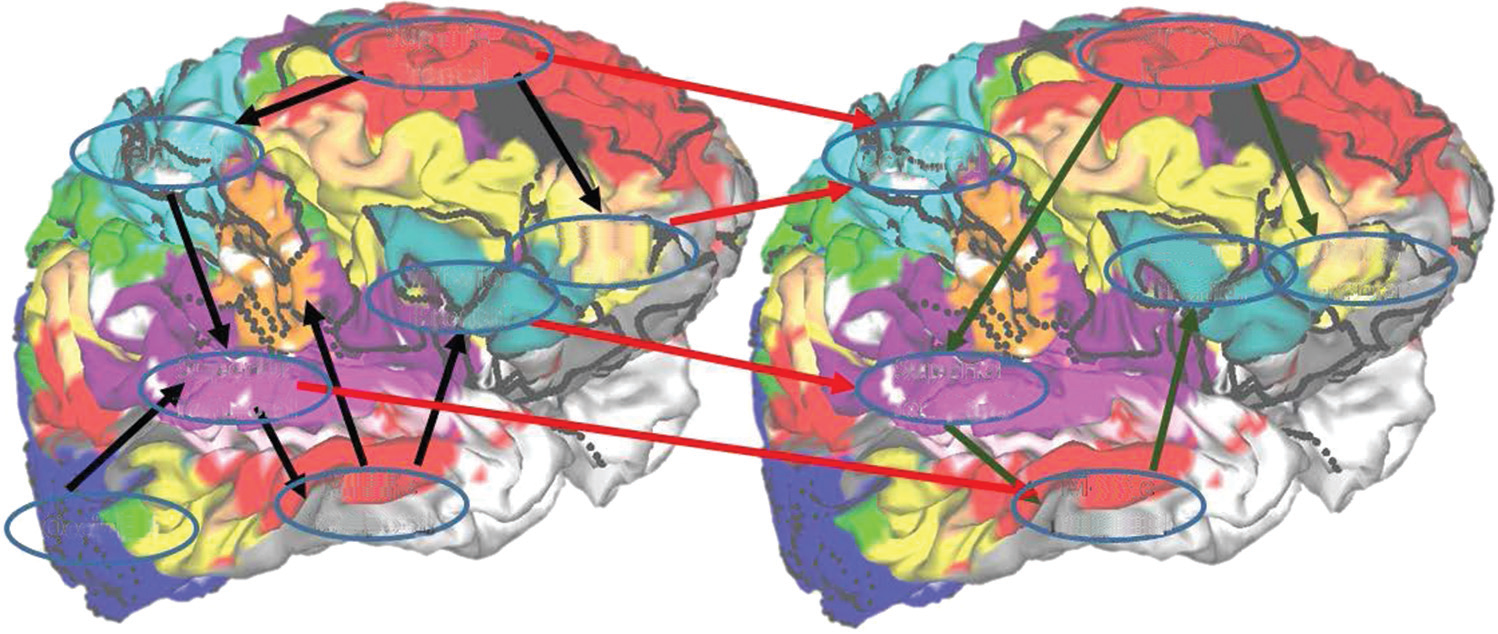
\includegraphics[width=14cm]{figures/ch06_figure15_data.png}};
\node[font=\scriptsize,fill=white,fill opacity=.88,text opacity=1,inner sep=1pt] at (4.1402,5.4766) {额上区};
\node[font=\scriptsize,fill=white,fill opacity=.88,text opacity=1,inner sep=1pt] at (1.5888,4.5234) {中央区};
\node[font=\scriptsize,fill=white,fill opacity=.88,text opacity=1,inner sep=1pt] at (5.9346,3.6355) {眶额区};
\node[font=\scriptsize,fill=white,fill opacity=.88,text opacity=1,inner sep=1pt] at (4.3645,3.1589) {额下区};
\node[font=\scriptsize,fill=white,fill opacity=.88,text opacity=1,inner sep=1pt] at (2.2243,2.3084) {颞上区};
\node[font=\scriptsize,fill=white,fill opacity=.88,text opacity=1,inner sep=1pt] at (3.4860,1.1495) {颞中区};
\node[font=\scriptsize,fill=white,fill opacity=.88,text opacity=1,inner sep=1pt] at (0.9439,1.0093) {枕区};
\node[font=\scriptsize,fill=white,fill opacity=.88,text opacity=1,inner sep=1pt] at (11.1869,5.4579) {额上区};
\node[font=\scriptsize,fill=white,fill opacity=.88,text opacity=1,inner sep=1pt] at (8.6449,4.4486) {中央区};
\node[font=\scriptsize,fill=white,fill opacity=.88,text opacity=1,inner sep=1pt] at (12.9439,3.4953) {眶额区};
\node[font=\scriptsize,fill=white,fill opacity=.88,text opacity=1,inner sep=1pt] at (11.1589,3.3178) {额下区};
\node[font=\scriptsize,fill=white,fill opacity=.88,text opacity=1,inner sep=1pt] at (8.9346,2.3178) {颞上区};
\node[font=\scriptsize,fill=white,fill opacity=.88,text opacity=1,inner sep=1pt] at (10.3738,1.1495) {颞中区};
\node at (3.5,-.35) {$T_0$};\node at (10.5,-.35) {$T_1$};
\end{tikzpicture}
\origfig{15}{fMRI 的有效连接图。}
\end{figure}


\section{因果机器学习}

当前疾病风险预测与关联分析的范式，是使用非结构化变量进行分类与检验（Sun et al. 2014），对结构化数据的关注较少（Wu et al. 2015）。然而，因果网络提供复杂疾病遗传、表观遗传与影像结构的整体视图。传统机器学习方法通常探索变量间的统计关联以作预测，较少考虑潜在的数据生成过程（Gershman and Daw 2017）。现实世界中的预测系统不断变化，训练数据与测试数据的分布经常显著不同。影像数据为系统潜在状态提供的信息并不完备。常用影像—基因组数据分析模型不考虑数据生成机制。我们经常发现，利用影像数据在训练集上预测准确，在测试集上却不理想。没有因果知识，常会选出无法泛化到测试场景的特征，导致预测不准（Magliacane et al. 2017）。

因果机器学习（causal machine learning，CML）的目标，是探索数据生成过程潜在的因果结构，用于特征选择与分类。为利用这种因果结构，先为因果图建立恰当的特征表示，再发展稀疏充分降维（sufficient dimension reduction，SDR），对因果图作特征选择（Mairal and Yu 2013）。SDR 是一种同时利用遗传信息与疾病信息的监督降维方法。它在不损失分类所需疾病信息的前提下，选择原始预测变量线性组合的最小集合（Chen et al. 2010）。

考虑 DAG $G=(V,E)$，其中 $V=\{x_1,\ldots,x_k\}$，$E=\{E_j,j=1,\ldots,m\}$，$E_j=\{(x_{a_j},x_{b_j})\mid x_{a_j},x_{b_j}\in V\}$，可用 6.5 节及本书其他章节讨论的因果推断方法推断。对 DAG 的节点排序，利用全部节点和边的信息，为 DAG 定义新的特征向量
\[
X=[x_1,\ldots,x_k,x_{a_1}x_{b_1},\ldots,x_{a_m}x_{b_m}]^T.
\]
令 $\Upsilon$ 为个体类别标签。SDR 寻找线性子空间 $S$，使响应 $\Upsilon$ 仅通过子空间 $S$ 中的向量依赖于 $X$，记为 $S_{\Upsilon\mid X}$。令 $B=[\beta_1,\ldots,\beta_d]$ 为构成 $S_{\Upsilon\mid X}$ 的基矩阵。为最大限度地利用降维空间中的信息，求解以下优化问题（Wang T and Zhu 2013）：
\begin{equation}
\min_\beta E\bigl[\lVert T_i(\Upsilon)-E(T_i(\Upsilon))-(X-E(X))^T\beta\rVert_2^2\bigr],
\tag{6.242}
\end{equation}
其中，$T_i(y)$ 相互正交，是泛函 $y$ 的一组变换函数。利用变换函数的基函数展开，上述问题可转化为最优评分问题（Clemmensen et al. 2011）。SDR 的最优评分表述对小问题效果良好，但特征数很大时会遇到困难。为解决这一问题，进一步将最优评分问题转化为
\begin{equation}
|\Upsilon\theta_i-X\beta_i\rVert_2^2+\lambda\sum_l|\beta_l^*\rVert_2^{1-r}
\quad\text{s.t. }\theta_i^TD\theta_i=1,\quad\theta_i^TD\theta_j=0,
\tag{6.243}
\end{equation}
其中，$B=[\beta_1,\ldots,\beta_i]=[\beta_1^*,\ldots,\beta_p^*]^T$，并用 ADMM（Boyd et al. 2011）求解。

\Needspace{4\baselineskip}
\noindent\textbf{例 6.7}

为验证因果机器学习用于风险预测的可行性，进行一项先导研究：将所提 CML 应用于精神分裂症（schizophrenia，SCZ）影像与基因组数据集，其中 64 名 SCZ 患者和 78 名健康对照共有 142 组 DTI，以及 14,412 个基因（746,575 个 SNP）的分型数据。采用五折交叉验证评价准确率。表 6.1 给出五折的平均结果。
\begin{table}[htbp]
\centering
\origtable{1}{利用 CML 与其他方法预测 SCZ 的准确率}
\small\setlength{\tabcolsep}{5pt}
\begin{tabular}{lrrrrrr}
\toprule
&\multicolumn{3}{c}{训练集}&\multicolumn{3}{c}{测试集}\\
\cmidrule(lr){2-4}\cmidrule(lr){5-7}
方法&准确率&灵敏度&特异度&准确率&灵敏度&特异度\\
\midrule
CML&1&1&1&0.951&0.962&0.939\\
仅 MPCA&0.989&0.994&0.984&0.542&0.48&0.619\\
MPCA SDR&0.977&0.959&0.99&0.611&0.307&0.845\\
仅 FPC&0.984&0.975&0.983&0.574&0.089&0.952\\
FPC SDR&0.986&0.983&0.986&0.662&0.515&0.793\\
\bottomrule
\end{tabular}
\end{table}

五折均选中共 11 个脑子区域，其中 7 个子区域与基因显著连接，$P$ 值小于 $3.5\mathrm{E}{-06}$。发现调控差异表达 miRNA、并与 SCZ 关联的基因 ALDOA，与能够高准确率预测 SCZ 的脑区域相连。表 6.1 表明，CML 在测试集中的平均预测准确率远高于其他方法，具有很强的泛化能力。CML 分析可计算每个区域的分类准确率。例如，脑子区域可按分类准确率排序为：MOG（左）（0.672）、SCC（0.651）、MOG（右）（0.648）、PG（左）（0.647）、SG（0.634）和 DT（0.621）；括号中数字为测试集五折的平均分类准确率。这说明，有些方法使用单个脑区域，可能比使用全部脑影像信息获得更高准确率。据报道，MOG（Takahashi et al. 2011）、SCC（Balevich et al. 2015）、PG（Brauns et al. 2015）及 DT（Pergola et al. 2015）的功能与结构异常，对 SCZ 的病理生理有贡献。

\section*{软件包}
\addcontentsline{toc}{section}{软件包}

U-Net：用于生物医学图像分割的卷积网络，其软件可从以下网址下载：
\url{https://lmb.informatik.uni-freiburg.de/people/ronneber/u-net/}。

所有模型均用 Caffe，在单块 NVIDIA Tesla K40c 上训练与测试。模型与代码公开于
\url{http://fcn.berkeleyvision.org}。

基于条件随机场的语义分割代码可从以下网址下载：
\url{https://github.com/Vaan5/piecewisecrf}。

DeconvNet 用于学习语义分割的反卷积网络，其软件可从以下网址下载：
\url{https://github.com/HyeonwooNoh/DeconvNet}。
